% Dokumentklassen s�ttes til memoir.
% Manual: http://ctan.org/tex-archive/macros/latex/contrib/memoir/memman.pdf
\documentclass[a4paper,oneside,article]{memoir}

\usepackage{pgf}
\usepackage{tikz}
\usepackage{pgfplots}
\usetikzlibrary{arrows,automata}
\usepackage{verbatim}
 
% Danske udtryk (fx figur og tabel) samt dansk orddeling og fonte med
% danske tegn. Hvis LaTeX brokker sig over �, � og � skal du udskifte
% "utf8" med "latin1" eller "applemac". 
\usepackage{inputenc}
\usepackage[danish]{babel}
\usepackage[T1]{fontenc}
 
% Matematisk udtryk, fede symboler, theoremer og fancy ting (fx k�debr�ker)
\usepackage{amsmath,amssymb}
\usepackage{bm}
\usepackage{amsthm}
%\usepackage{mathtools}
 
% Kodelisting. Husk at l�se manualen hvis du vil lave fancy ting.
% Manual: http://mirror.ctan.org/macros/latex/contrib/listings/listings.pdf
\usepackage{listings}
 
% Fancy ting med enheder og datatabeller. L�s manualen til pakken
% Manual: http://www.ctan.org/tex-archive/macros/latex/contrib/siunitx/siunitx.pdf
%\usepackage{siunitx}

% Inds�ttelse af grafik.
\usepackage{graphicx}
\usepackage{float}
\usepackage{caption}
\usepackage{subcaption}
 
% Reaktionsskemaer. L�s manualen for at se eksempler.
% Manual: http://www.ctan.org/tex-archive/macros/latex/contrib/mhchem/mhchem.pdf
%\usepackage[version=3]{mhchem}
%\usepackage[noend]{algpseudocode}
%\usepackage{algorithm}

\usepackage{xcolor,colortbl}

\usepackage{listings}

\definecolor{javared}{rgb}{0.6,0,0} % for strings
\definecolor{javagreen}{rgb}{0.25,0.5,0.35} % comments
\definecolor{javapurple}{rgb}{0.5,0,0.35} % keywords
\definecolor{javadocblue}{rgb}{0.25,0.35,0.75} % javadoc

\lstset{language=Java,
basicstyle=\small, %\ttfamily,
keywordstyle=\color{javapurple}\bfseries,
stringstyle=\color{javared},
commentstyle=\color{javagreen},
morecomment=[s][\color{javadocblue}]{/**}{*/},
numbers=left,
numberstyle=\tiny\color{black},
stepnumber=1,
numbersep=10pt,
tabsize=4,
showspaces=false,
showstringspaces=false}

\newcommand{\notimplies}{%
  \mathrel{{\ooalign{\hidewidth$\not\phantom{=}$\hidewidth\cr$\implies$}}}}

\begin{document}
    \title{Reliable Group Communication - Disposition}
    \author{Lukas Peter J�rgensen, 201206057, DA4
            }
    \maketitle
    
    \chapter{Intro}
    Guarantee that messages are delivered to all members in a process group.\\
    \textbf{Naive solution} $\rightarrow$ endless iteration.
    \section*{Issues}
    Simple case: simply have $n$ point-to-point channels.
    \begin{itemize}
    \item May waste network bandwidth, might be an issue in large networks.
    \item Limited by number of channels.
    \end{itemize}
    \chapter{Reliable multicasting}
    \textbf{Intuitively:} A message sent to a group, should be delivered to each member of that group.\\
    \textbf{What if:} A process joins during communication? Or a (sending) process crashes during communication.\\
    \\
    \textbf{Distinction} between two cases. Reliable communication in the presence of faulty processes, and reliable communication when processes are assumed to operate correctly.\\
    In the first case, multicasting is considered to be reliable when all nonfaulty group members recieve the message.\\
    \\
    \textbf{First we will look at the second case, when we assume processes operate correctly.}
    \chapter{Simple solution}
    \textbf{Assumptions:} All receivers known and assumed not to fail.
    \begin{figure}[H]
    \centering
    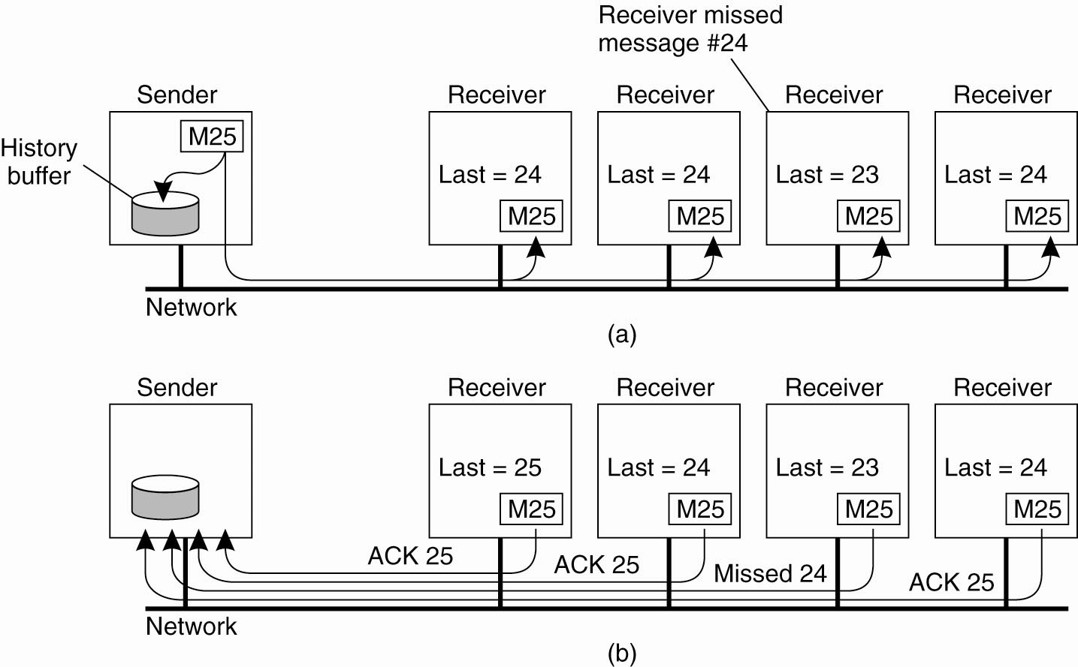
\includegraphics[width=\textwidth]{Media/RelMulti.jpg}
    \end{figure}
    \section*{Problem}
    \textbf{Cannot support large number of receivers.} If there are $N$ receivers, the sender must be prepared to accept at least $N$ acknowledgements. Sender may be swamped by acknowledgements. (Feedback implosion)\\
    \section*{Possible solutions}
    \textbf{Only feedback when something goes wrong}, what if the message is lost before reaching any of the users? Feedback implosion might still happen, sender will be forced to keep messages in it's buffer forever because it can never know if everyone has received the message.
    
    \chapter{Non-hierarchical}
    Scales reasonably well, has seen practical uses.
    \begin{figure}[H]
    \centering
    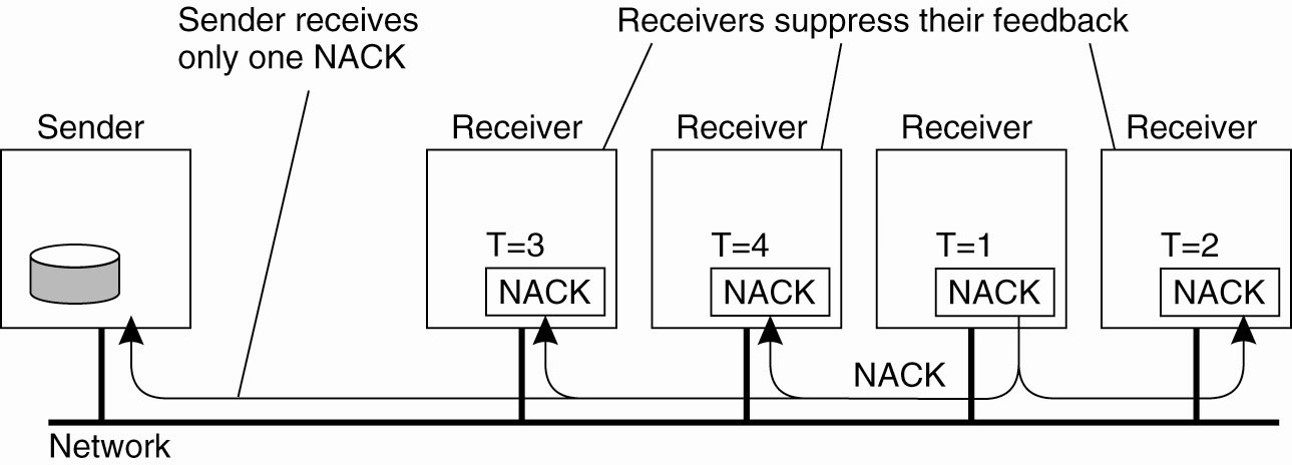
\includegraphics[width=\textwidth]{Media/NonHieMulti.jpg}
    \end{figure}
    If a process realizes it is missing a package, multicast the retransmission request.\\ 
    \textbf{But,} do it after a short random delay to avoid concurrent retransmission request, if a process needs a retransmission but has recieved a retransmission request from another receiver, it will simply suppress its own request.
    
    \section*{Problems}
    \textbf{Receivers have to process useless messages.} Whenever a retransmission request or a retransmission occurs, all receivers have to process the request even when it has nothing to do with them.\\
    \textbf{Ensuring that each feedback message is only sent once}, is a tricky issue as well?
         
    \chapter{Hierarchical}
    Scalability for large groups of receivers.
    \begin{figure}[H]
    \centering
    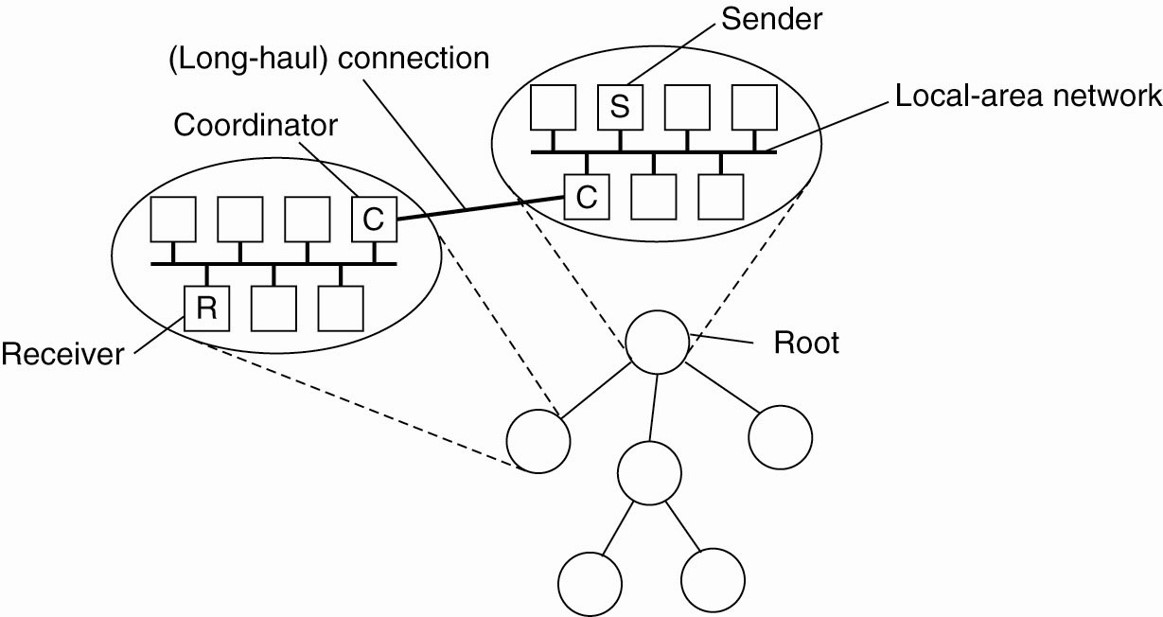
\includegraphics[width=\textwidth]{Media/HieMulti.jpg}
    \end{figure}
    Partition receivers into a number of subgroups, which can be organized into a tree.\\
    Each subgroup has a \textbf{coordinator} which is responsible for handling retransmission requests of receivers contained in its subgroup.\\
    In a scheme based on acknowledgements, each coordinator can delete a message $m$ from it's buffer when it has received acknowledgements for message $m$ from all members in its subgroup, as well as from its children.\\
    \textbf{Note:} Doesn't have to get acknowledgements from all children before it can send acknowledgement to its parent.
    
    \section*{Problems}
    \textbf{Construction of the tree,} is an issue as many cases need the tree to be constructed dynamically. One approach is to use the multicast tree in the underlying network, if there is one.\\
    \textbf{Principally,} the approach is to enhance each multicast router in the network layer such that it can act as a local coordinator. Unfortunately, as a practical matter such adaptations to existing networks are not easy to do, therefore application-level multicasting solutions have gained popularity.\\
    \\
    \textbf{Now we will look at the case in which we need to achieve reliable multicasting in the presence of process failures.}
    
    \chapter{Virtual Synchrony}
    It's important in the case where a process crashes during the execution of an update, hence missing that update and the other updates, while the other received the updates.\\
    The other processes should therefore de
    
\end{document}